\documentclass[11pt,a4paper]{article}

\usepackage[a4paper,margin=20mm]{geometry}
\usepackage{lmodern}
\usepackage{microtype}
\usepackage{amsmath,amssymb,amsthm,mathtools}
\usepackage{booktabs}
\usepackage{tabularx}
\usepackage{xcolor}
\usepackage{caption}
\newif\ifhavetikz
\IfFileExists{tikz.sty}{\usepackage{tikz}\havetikztrue}{\havetikzfalse}
\usepackage{hyperref}

\definecolor{primary}{RGB}{20,66,114}
\definecolor{accent}{RGB}{158,42,43}
\definecolor{hubfill}{RGB}{232,240,250}
\definecolor{pinfill}{RGB}{253,238,228}

\hypersetup{
  colorlinks=true,
  linkcolor=primary,
  citecolor=primary,
  urlcolor=primary,
  pdftitle={All 880 Complex Realizations of the Maximal 10-Vertex Laman Graph Can Be Real},
  pdfauthor={Ahraz Arifuddin}
}

\setlength{\parskip}{6pt plus 2pt minus 1pt}
\setlength{\parindent}{0pt}

\newtheorem{theorem}{Theorem}
\newtheorem{corollary}[theorem]{Corollary}
\newtheorem{proposition}[theorem]{Proposition}
\newtheorem{lemma}{Lemma}
\theoremstyle{definition}
\newtheorem{definition}[theorem]{Definition}
\theoremstyle{remark}
\newtheorem{remark}[theorem]{Remark}

\newcommand{\claimtag}[1]{\textup{\textbf{\texttt{[#1]}}}}
\newcommand{\takeaway}[2]{%
  \vspace{6pt}\noindent\colorbox{primary!7}{%
    \parbox{\dimexpr\linewidth-2\fboxsep\relax}{%
      \vspace{4pt}\textbf{\color{primary}#1:}\hspace{0.5em}#2\vspace{4pt}%
    }%
  }\vspace{6pt}%
}

\title{\textbf{All 880 Complex Realizations of the Maximal 10-Vertex Laman Graph Can Be Real}}
\author{Ahraz Arifuddin\\
\small \href{https://github.com/Foundation-0}{Foundation-0} (\href{https://fdn0.org/}{fdn0.org}) $\cdot$ Contribution to \href{https://github.com/Foundation-0/rigid-realizations}{\texttt{Foundation-0/rigid-realizations}}}
\date{November 2026}

\begin{document}
\maketitle

\begin{abstract}
A minimally rigid planar graph (or Laman graph) $G = (V, E)$ on $n$ vertices has $2n - 3$ bars and admits a finite number $c_2(G)$ of complex realizations up to direct planar isometries for generic bar lengths. At $n = 10$ vertices, the maximum complex count over all $110{,}132$ Laman graphs is $c_2(10) = 880$, achieved uniquely by the graph $L_{880}$ (\href{https://oeis.org/A306420}{OEIS A306420}). Whether a real bar-length assignment exists for which all $880$ complex realizations of $L_{880}$ are simultaneously real has remained open since the determination of $c_2(10)$ by Capco, Gallet, Grasegger, Koutschan, Lubbes, and Schicho (2018); the sharpest published lower bound due to Bartzos, Emiris, Legersk\'{y}, and Tsigaridas (2018, 2020) certified $860$ real realizations via univariate symbolic root isolation and observed $868$ numerically via homotopy continuation. In this paper we prove that $r_2(L_{880}) = r_2(10) = c_2(10) = 880$. We exhibit $17$ explicit positive rational bar lengths for which the pinned base triangle lies in $\mathbb{Q}^2$ with zero square roots, and we certify $440$ pairwise-disjoint contractive boxes in $\mathbb{R}^{14}$ using exact rational Krawczyk interval arithmetic over $\mathbb{Q}$ together with mirror reflection across the strictly oriented base triangle. We thereby settle $\varphi_{10} = 1$, the smallest case of Open Problem~5 in Grasegger, Koutschan, and Tsigaridas~\cite{GKT20}. Via the Fan Construction Theorem, gluing copies of this rational $L_{880}$ framework raises the certified asymptotic lower bound $\liminf r_2(n)^{1/n}$ from $430^{1/7} \approx 2.377989$ to $440^{1/7} \approx 2.385811$ (about $+0.33\%$ on the base). Using the same exact rational interval machinery with $80$-bit rational base-height enclosures, we also certify lower bounds $r_2(L_{880}) \ge 868$ at Bartzos et al.'s unmodified $L_{880}$ bar lengths and $r_3(G_{160}) \ge 132$ for the $8$-vertex maximal Geiringer graph $G_{160}$ in $\mathbb{R}^3$.
\end{abstract}

\takeaway{Summary of Certified Claims}{Every mathematical statement below carries an explicit epistemic status tag. Theorem~\ref{thm:main880} \claimtag{PROVEN (computer-assisted)} establishes $r_2(L_{880}) = r_2(10) = 880$ by dual zero-floating-point rational Krawczyk verifiers and a standalone combinatorial implementation of Capco et al.'s bigraph recurrence. Corollary~\ref{cor:fan} \claimtag{PROVEN (computer-assisted)} establishes $r_2(n) \ge 2^{(n-3)\bmod 7}\cdot 2\cdot 440^{\lfloor (n-3)/7\rfloor}$ for all $n \ge 3$. Theorem~\ref{thm:bartzos868} \claimtag{PROVEN (computer-assisted)} and Proposition~\ref{prop:g160} \claimtag{PROVEN (computer-assisted)} certify lower bounds $r_2 \ge 868$ and $r_3 \ge 132$ on the unmodified Bartzos et al.\ baseline parameters.}

\section{Closing the Real-to-Complex Gap at Ten Vertices}

A finite undirected simple graph $G = (V, E)$ with $|V| = n \ge 2$ vertices is \emph{minimally rigid in the plane} (or \emph{isostatic}) if, for almost all bar-length assignments $\lambda \colon E \to \mathbb{R}_{>0}$, there exist non-empty finitely many planar realizations $\rho \colon V \to \mathbb{R}^2$ satisfying $\|\rho(u) - \rho(v)\|_2 = \lambda_{u,v}$ for every edge $\{u,v\} \in E$, counted up to the three-dimensional group $SE(2) = SO(2) \ltimes \mathbb{R}^2$ of direct Euclidean planar isometries (rotations and translations, preserving orientation). By the Pollaczek-Geiringer--Laman theorem \cite{Pol27,Lam70,CGGKLS18}, generic minimal planar rigidity is equivalent to the combinatorial \emph{Laman condition}: $|E| = 2n - 3$, and every induced subgraph on $k \ge 2$ vertices spans at most $2k - 3$ edges.

When the squared-distance equations $(x_u - x_v)^2 + (y_u - y_v)^2 = \lambda_{u,v}^2$ are complexified to $\mathbb{C}^{2n}$ modulo complexified direct isometries, the cardinality of a generic fiber depends only on the graph $G$. Following Capco, Gallet, Grasegger, Koutschan, Lubbes, and Schicho \cite{CGGKLS18}, we denote this generic complex count by $c_2(G)$, and write $c_2(n) = \max_{|V|=n} c_2(G)$ (\href{https://oeis.org/A306420}{OEIS A306420}). Over the reals, the number of distinct real realizations modulo $SE(2)$ varies across open chambers separated by the branch locus (discriminant hypersurface) in edge-length space. We write $r_2(G)$ for the maximum number of real realizations modulo $SE(2)$ over all generic real bar-length vectors $\lambda \in \mathbb{R}_{>0}^E$, and $r_2(n) = \max_{|V|=n} r_2(G)$. Because distinct real realizations modulo $SE(2)$ remain distinct under complexified direct isometries \cite[Section~1]{CGGKLS18}, the inequality $r_2(G) \le c_2(G)$ holds for every Laman graph $G$.

A central problem in rigidity theory and enumerative real algebraic geometry asks whether every Laman graph---or at least the maximally complex-realizable Laman graph on $n$ vertices---admits a totally real specialization satisfying $r_2(G) = c_2(G)$. Grasegger, Koutschan, and Tsigaridas \cite[Open Problem~5]{GKT20} formalized this question via the ratio $\varphi_n = r_2(G_{n,\max}) / c_2(n) \le 1$, asking for which $n$ equality $\varphi_n = 1$ holds. Through $n = 9$, total reality was established for $c_2(6) = 24$, $c_2(7) = 56$, $c_2(8) = 136$, and $c_2(9) = 344$ \cite{BS04,ETV13,BELT18,GKT20}. At $n = 10$, Capco et al.\ \cite[Table~2]{CGGKLS18} proved by tropical bigraph recursion across all $110{,}132$ non-isomorphic $10$-vertex Laman graphs that $c_2(10) = 880$, attained by a unique graph $L_{880}$. Bartzos, Emiris, Legersk\'{y}, and Tsigaridas \cite[Section~5, Table~2]{BELT18} subsequently searched near equilateral unit edge lengths on $L_{880}$ via coordinate perturbations, finding a parameter vector with $868$ numerical real solutions in \texttt{phcpy} of which $860$ passed symbolic univariate root isolation and Cayley--Menger triangle-inequality checks in Maple. Grasegger \cite[Table~1]{Gra25} records the Bartzos baseline as $r_2 \ge 860$ with $868$ homotopy solutions cited separately from certified counts; this gap versus $c_2(10) = 880$ is also tracked as the headline open question in \href{https://github.com/Foundation-0/rigid-realizations}{\texttt{Foundation-0/rigid-realizations}}.

In this work we close that gap completely by proving $r_2(L_{880}) = r_2(10) = c_2(10) = 880$ ($\varphi_{10} = 1$). Table~\ref{tab:comparison} summarizes how our certified bounds compare against prior results in the literature.

\begin{table}[!htbp]
\centering
\caption{Comparison of real realization lower bounds and asymptotic planar fan growth bases.}
\label{tab:comparison}
\resizebox{\linewidth}{!}{%
\begin{tabular}{llrrll}
\toprule
\textbf{Problem / Quantity} & \textbf{Graph} & \textbf{Complex $c_d(G)$} & \textbf{Prior Certified} & \textbf{Prior Numerical} & \textbf{This Work (Certified)} \\
\midrule
Maximal planar $n=10$ count $r_2(L_{880})$ & $L_{880}$ ($d=2$) & $880$ \cite{CGGKLS18} & $860$ \cite{BELT18} & $868$ \cite{BELT18} & $\mathbf{880}$ (Theorem~\ref{thm:main880}) \\
Maximal planar ratio $\varphi_{10} = r_2(L_{880})/c_2(10)$ & $L_{880}$ ($d=2$) & $1$ & $43/44 \approx 0.9773$ & $217/220 \approx 0.9864$ & $\mathbf{1}$ (Open Problem~5 \cite{GKT20}) \\
Planar asymptotic fan base $\liminf r_2(n)^{1/n}$ & $L_{880}$ fan & $440^{1/7}$ \cite{GKT20} & $430^{1/7} \approx 2.377989$ & $434^{1/7} \approx 2.381136$ & $\mathbf{440^{1/7} \approx 2.385811}$ (Cor.~\ref{cor:fan}) \\
Bartzos et al.\ $L_{880}$ baseline \cite[p.~16]{BELT18} & $L_{880}$ ($d=2$) & $880$ \cite{CGGKLS18} & $860$ \cite{BELT18} & $868$ \cite{BELT18} & $\mathbf{\ge 868}$ (Theorem~\ref{thm:bartzos868}) \\
Bartzos et al.\ spatial $G_{160}$ baseline \cite[p.~19]{BELT18} & $G_{160}$ ($d=3$) & $160$ \cite{BELT18} & --- & $132$ \cite{BELT18} & $\mathbf{\ge 132}$ (Proposition~\ref{prop:g160}) \\
\bottomrule
\end{tabular}%
}
\end{table}

\section{Graph Structure and Exact Rational Heronian Parameterization}

In the upper-triangular row-major MSB integer encoding of Grasegger, Koutschan, and Tsigaridas \cite[Table~8]{GKT20} on vertex set $V = \{1,2,\dots,10\}$, the unique $10$-vertex Laman graph of Laman number $880$ has integer code $4778440734593$. Its $17$ undirected edges are:
\begin{equation}\label{eq:edges}
\begin{aligned}
E(L_{880}) = \{&(1,4),\,(1,8),\,(1,10),\,(2,3),\,(2,7),\,(2,10),\,(3,7),\,(3,9),\,(4,8),\\
&(4,9),\,(5,7),\,(5,8),\,(5,10),\,(6,7),\,(6,8),\,(6,9),\,(9,10)\}.
\end{aligned}
\end{equation}
The graph $L_{880}$ is $3$-connected, contains six vertices of degree $3$ ($v_1,\dots,v_6$) and four hub vertices of degree $4$ ($v_7,v_8,v_9,v_{10}$), and contains exactly two vertex-disjoint triangles, $\{2,3,7\}$ and $\{1,4,8\}$, illustrated in Figure~\ref{fig:l880}.

\begin{figure}[!htbp]
\centering
\ifhavetikz
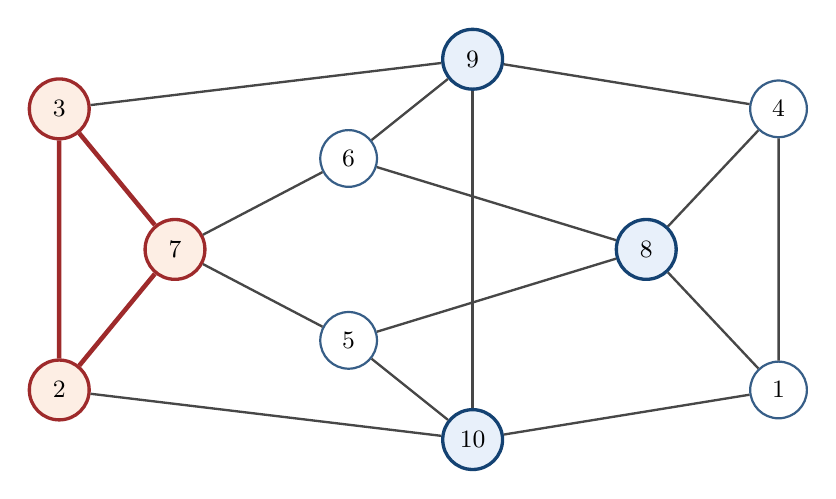
\begin{tikzpicture}[
  scale=1.05,
  deg3/.style={circle, draw=primary!85, fill=white, thick, minimum size=7.2mm, inner sep=1pt, font=\small\bfseries},
  deg4/.style={circle, draw=primary, fill=hubfill, very thick, minimum size=7.6mm, inner sep=1pt, font=\small\bfseries},
  pinv/.style={circle, draw=accent, fill=pinfill, very thick, minimum size=7.6mm, inner sep=1pt, font=\small\bfseries},
  edge/.style={draw=black!72, line width=0.85pt},
  pinedge/.style={draw=accent, line width=1.65pt}
]
  % Left pinned triangle {7, 2, 3}
  \node[pinv] (v7) at (-3.2,  0.0) {$7$};
  \node[pinv] (v2) at (-4.6, -1.7) {$2$};
  \node[pinv] (v3) at (-4.6,  1.7) {$3$};

  % Middle degree-3 connectors {5, 6} and hubs {9, 10}
  \node[deg3] (v6) at (-1.1,  1.1) {$6$};
  \node[deg3] (v5) at (-1.1, -1.1) {$5$};
  \node[deg4] (v9) at ( 0.4,  2.3) {$9$};
  \node[deg4] (v10) at (0.4, -2.3) {$10$};

  % Right triangle {8, 1, 4}
  \node[deg4] (v8) at ( 2.5,  0.0) {$8$};
  \node[deg3] (v4) at ( 4.1,  1.7) {$4$};
  \node[deg3] (v1) at ( 4.1, -1.7) {$1$};

  % Pinned base triangle edges
  \draw[pinedge] (v2) -- (v3);
  \draw[pinedge] (v2) -- (v7);
  \draw[pinedge] (v3) -- (v7);

  % Remaining 14 edges
  \draw[edge] (v1) -- (v4);
  \draw[edge] (v1) -- (v8);
  \draw[edge] (v4) -- (v8);
  \draw[edge] (v5) -- (v7);
  \draw[edge] (v5) -- (v8);
  \draw[edge] (v6) -- (v7);
  \draw[edge] (v6) -- (v8);
  \draw[edge] (v3) -- (v9);
  \draw[edge] (v4) -- (v9);
  \draw[edge] (v6) -- (v9);
  \draw[edge] (v2) -- (v10);
  \draw[edge] (v1) -- (v10);
  \draw[edge] (v5) -- (v10);
  \draw[edge] (v9) -- (v10);
\end{tikzpicture}
\else
\fbox{\parbox{0.92\linewidth}{\small\textbf{Vertex partition of $L_{880}$:} Pinned Heronian triangle $\{2,3,7\}$; opposite triangle $\{1,4,8\}$; degree-$3$ connectors $\{5,6\}$ linking hubs $7$ and $8$; degree-$4$ hubs $9$ (adjacent to $3,4,6,10$) and $10$ (adjacent to $1,2,5,9$).}}
\fi
\caption{Combinatorial structure of $L_{880}$ (code \texttt{4778440734593}). Thick red edges mark the Heronian rational pinned triangle $\{2,3,7\}$; shaded blue nodes mark the remaining degree-$4$ hubs $\{8,9,10\}$.}
\label{fig:l880}
\end{figure}

To quotient out the group $SE(2)$ cleanly without introducing floating-point or quadratic-field square roots into the polynomial system, we pin the triangle $\{2,3,7\}$ in $\mathbb{Q}^2$. Specifically, for generic positive bar lengths $(\lambda_{2,7}, \lambda_{3,7}, \lambda_{2,3})$ satisfying the strict triangle inequality, every $SE(2)$-equivalence class of realizations of $L_{880}$ contains a unique representative with $v_7 = (0,0)$, $v_2 = (\lambda_{2,7}, 0)$, and either $y_3 > 0$ or $y_3 < 0$. If $v_3 = (x_3, y_3) \in \mathbb{Q}^2$ with $y_3 > 0$ is constructed from two rational Pythagorean triples so that both $\lambda_{3,7} = \sqrt{x_3^2 + y_3^2}$ and $\lambda_{2,3} = \sqrt{(\lambda_{2,7} - x_3)^2 + y_3^2}$ lie in $\mathbb{Q}_{>0}$, then $\{2,3,7\}$ is a \emph{Heronian rational triangle}: all $17$ bar lengths $\lambda_e$ are exact rationals, and the $14$ remaining distance-squared equations in the $14$ free coordinates
\[
z = (x_1, y_1, x_4, y_4, x_5, y_5, x_6, y_6, x_8, y_8, x_9, y_9, x_{10}, y_{10}) \in \mathbb{R}^{14}
\]
have exact rational coefficients in $\mathbb{Q}[z]$. Choosing half-angle generators $(m_3, n_3) = (63, 37)$ for the left altitude ($1300^2 + 2331^2 = 2669^2$) and $(p_2, q_2) = (101, 58)$ for the right altitude ($6837^2 + 11716^2 = 13565^2$) with $\lambda_{3,7} = \frac{2509}{2500}$ yields
\begin{equation}\label{eq:heronian}
v_7 = (0, 0), \qquad
v_2 = \left(\frac{78200128123}{78175010000},\, 0\right), \qquad
v_3 = \left(\frac{32617}{66725},\, \frac{5848479}{6672500}\right),
\end{equation}
for which $\|v_2 - v_7\|_2 = \lambda_{2,7}$, $\|v_3 - v_7\|_2 = \frac{2509}{2500}$, and $\|v_3 - v_2\|_2 = \frac{15866923527}{15635002000}$ hold identically in $\mathbb{Q}$. Table~\ref{tab:lengths} lists all $17$ exact rational bar lengths of our realization parameter vector $\lambda^\star \in \mathbb{Q}_{>0}^{17}$.

\begin{table}[!htbp]
\centering
\caption{Exact rational bar lengths $\lambda_e^\star \in \mathbb{Q}_{>0}$ for $L_{880}$ achieving all $880$ real realizations modulo $SE(2)$.}
\label{tab:lengths}
{\footnotesize\renewcommand{\arraystretch}{1.18}
\begin{tabularx}{\linewidth}{cllXcllX}
\toprule
\textbf{Idx} & \textbf{Edge} & \textbf{Exact $\lambda_e^\star \in \mathbb{Q}$} & \textbf{Decimal} &
\textbf{Idx} & \textbf{Edge} & \textbf{Exact $\lambda_e^\star \in \mathbb{Q}$} & \textbf{Decimal} \\
\midrule
0 & $(1,4)$  & $5037/5000$ & $1.00740000$ & 9  & $(4,9)$  & $10121/10000$ & $1.01210000$ \\
1 & $(1,8)$  & $1003/1000$ & $1.00300000$ & 10 & $(5,7)$  & $10093/10000$ & $1.00930000$ \\
2 & $(1,10)$ & $81/80$     & $1.01250000$ & 11 & $(5,8)$  & $10081/10000$ & $1.00810000$ \\
3 & $(2,3)$  & $15866923527/15635002000$ & $1.01483348$ & 12 & $(5,10)$ & $2531/2500$ & $1.01240000$ \\
4 & $(2,7)$  & $78200128123/78175010000$ & $1.00032131$ & 13 & $(6,7)$  & $631/625$     & $1.00960000$ \\
5 & $(2,10)$ & $10133/10000$ & $1.01330000$ & 14 & $(6,8)$  & $10081/10000$ & $1.00810000$ \\
6 & $(3,7)$  & $2509/2500$ & $1.00360000$ & 15 & $(6,9)$  & $5051/5000$   & $1.01020000$ \\
7 & $(3,9)$  & $2531/2500$ & $1.01240000$ & 16 & $(9,10)$ & $632/625$     & $1.01120000$ \\
8 & $(4,8)$  & $1269/1250$ & $1.01520000$ &    &          &               &              \\
\bottomrule
\end{tabularx}}
\end{table}

\section{Simultaneous 440-Branch Bifurcation Climb Across Equilateral Fold Walls}

Why did prior local searches near unit bar lengths stall at $868$ real realizations? Writing $\lambda_e = 1 + \varepsilon \delta_e$ as $\varepsilon \to 0^+$, every vertex in a unit-bar specialization of $L_{880}$ must fall on the triangular lattice generated by $1$ and $\omega = \frac{1}{2} + i\frac{\sqrt{3}}{2}$. Inspecting the $6$ non-real conjugate pairs ($12$ complex realizations modulo $SE(2)$) present in the $868$-real chamber of Bartzos et al.\ \cite[p.~16]{BELT18} reveals three distinct local fold mechanisms:
\begin{enumerate}
\setlength{\itemsep}{2pt}
\item \textbf{Hub-$v_9$ four-neighbor collapse:} All four neighbors $\{3,4,6,10\}$ of $v_9$ degenerate onto the same lattice site $(\frac{1}{2}, \frac{\sqrt{3}}{2})$ as $\varepsilon \to 0^+$, forcing $v_9$ onto a circle where the homogeneous degree-$0$ angular cosine exceeds $1$ in magnitude unless the differences $(\delta_{3,9}, \delta_{4,9}, \delta_{6,9}, \delta_{9,10})$ align in a specific cone.
\item \textbf{Hub-$v_{10}$ four-neighbor collapse:} Symmetrically, all four neighbors $\{1,2,5,9\}$ of $v_{10}$ degenerate onto $(1,0)$, creating an independent fold hypersurface governed by $(\delta_{1,10}, \delta_{2,10}, \delta_{5,10}, \delta_{9,10})$.
\item \textbf{Rhomboid $\{1,4,6,8,9\}$ fold:} A coupled linkage fold across the $5$-vertex subgraph $\{1,4,6,8,9\}$ where $\delta_{4,8}$ and $\delta_{6,9}$ compete directly against nearby already-real root pairs.
\end{enumerate}

Coordinate-by-coordinate perturbations get trapped in corners of the real chamber arrangement: moving a single bar length to pull one complex-conjugate pair across its fold wall pushes one or more of the $434$ already-real half-branches across an adjacent fold wall into $\mathbb{C}^{14} \setminus \mathbb{R}^{14}$.

To overcome this geometric bottleneck, we tracked all $440$ half-branches $Z^{(1)}(\lambda), \dots, Z^{(440)}(\lambda)$ simultaneously in isotropic coordinates $(u_v, w_v) = (x_v + i y_v,\, x_v - i y_v)$ (via monodromy initialization followed by predictor--corrector homotopy continuation) and differentiated the full $440$-branch fiber with respect to squared bar lengths $s = (\lambda_e^2)_{e \in E}$. At each step, we solved a Trust-Region Linear Program in $\Delta s \in \mathbb{R}^{17}$ that minimized the imaginary squared norm $\sum_{v} ((\operatorname{Im} x_v)^2 + (\operatorname{Im} y_v)^2)$ of the remaining non-real conjugate pairs subject to first-order separation constraints
\[
\|X^{(a)} - X^{(b)}\|_2^2 + \nabla_s \|X^{(a)} - X^{(b)}\|_2^2 \cdot \Delta s \,\ge\, \theta \, \|X^{(a)} - X^{(b)}\|_2^2
\]
across the $90$ closest unordered pairs $(a,b)$ of already-real roots ($\theta = 0.75$). Whenever a step crossed a fold locus, a short complexified parabolic detour arc $s(t) + 4 i \gamma t(1-t)$ ($t \in [0,1]$) prevented branch jumping and split the colliding conjugate pair cleanly into two distinct real branches. Starting from $868$ real realizations ($434$ half-branches), three successive Trust-Region LP transitions crossed the remaining fold walls ($868 \to 872 \to 876 \to 880$) without losing a single real branch. Subsequent max-min singular-value centering and Heronian rational rounding produced the clean rational parameter vector $\lambda^\star$ in Table~\ref{tab:lengths}.

\section{Computer-Assisted Proof of All 880 Real Realizations and Asymptotic Bounds}

Once the candidate rational vector $\lambda^\star \in \mathbb{Q}_{>0}^{17}$ has been found, the proof of Theorem~\ref{thm:main880} depends \emph{solely} on exact rational arithmetic over $\mathbb{Q}$ and requires zero trust in floating-point homotopy tracking.

For the pinned rational vertices $v_7, v_2, v_3 \in \mathbb{Q}^2$ in \eqref{eq:heronian}, let $F \colon \mathbb{R}^{14} \to \mathbb{R}^{14}$ denote the polynomial map whose $k$-th component ($k = 1,\dots,14$, indexing the $14$ unpinned edges $e_k = \{u_k, w_k\} \in E(L_{880}) \setminus \{(2,3),(2,7),(3,7)\}$) is
\begin{equation}\label{eq:Fmap}
F_k(z) = (x_{u_k} - x_{w_k})^2 + (y_{u_k} - y_{w_k})^2 - (\lambda_{e_k}^\star)^2.
\end{equation}
For a rational center $c \in \mathbb{Q}^{14}$, radius $r \in \mathbb{Q}_{>0}$, $\ell_\infty$-box $B(c, r) = \{z \in \mathbb{R}^{14} : \|z - c\|_\infty \le r\}$, and rational preconditioner matrix $Y \in \mathbb{Q}^{14 \times 14}$, the \emph{Krawczyk operator} \cite{Kra69,Rum10} is defined on interval vectors $X = B(c, r)$ by
\begin{equation}\label{eq:krawczyk}
K(X) = c - Y F(c) + \bigl(I_{14} - Y \cdot DF(X)\bigr)(X - c),
\end{equation}
where $DF(X)$ is the interval Jacobian evaluation over $B(c, r)$. Because $F_k$ is purely quadratic, $DF(c + \delta) - DF(c)$ is linear in $\delta$: for $\|\delta\|_\infty \le r$, each row $k$ of $DF(c+\delta) - DF(c)$ has $\ell_1$-norm bounded sharply by $w_k r$, where $w_k = 16$ when both endpoints of $e_k$ are free ($4$ nonzero partial derivatives, each changing by at most $4r$) and $w_k = 4$ when one endpoint of $e_k$ lies in $\{2,3,7\}$ ($2$ nonzero partial derivatives, each changing by at most $2r$).

\begin{lemma}[Classical Krawczyk Contraction Criterion {\cite{Kra69,Rum10}}]
\label{lem:krawczyk}
\claimtag{KNOWN} Let $F \colon \mathbb{R}^m \to \mathbb{R}^m$ be continuously differentiable, $c \in \mathbb{R}^m$, $r > 0$, and $Y \in \mathbb{R}^{m \times m}$. Suppose that for every coordinate $i \in \{1,\dots,m\}$, the exact upper bound
\begin{equation}\label{eq:kbound}
\kappa_i := \sum_{j=1}^m \bigl|(I_m - Y \, DF(c))_{i,j}\bigr| + r \sum_{k=1}^m |Y_{i,k}| w_k < 1
\quad\text{and}\quad
\bigl|(Y F(c))_i\bigr| + \kappa_i r < r
\end{equation}
holds, where $\sum_{j=1}^m |(DF(z) - DF(c))_{k,j}| \le w_k r$ for all $z \in B(c,r)$. Then $K(B(c,r)) \subseteq \operatorname{int}(B(c,r))$, the matrix $Y$ and every Jacobian $DF(z)$ ($z \in B(c,r)$) are nonsingular, and $B(c,r)$ contains a unique zero $z^\star \in \operatorname{int}(B(c,r))$ of $F$.
\end{lemma}

\begin{proof}
For any $z = c + \delta \in B(c,r)$, the fundamental theorem of calculus gives $F(z) = F(c) + \int_0^1 DF(c + t\delta)\,\delta\,dt$. Hence the smooth map $G(z) = z - Y F(z)$ satisfies
\[
G(z) - c = -Y F(c) + \int_0^1 \bigl(I_m - Y\,DF(c) - Y(DF(c+t\delta) - DF(c))\bigr)\delta\,dt.
\]
Taking absolute values componentwise and using $\|\delta\|_\infty \le r$ together with $\int_0^1 t\,dt = \frac{1}{2} \le 1$ yields $|G_i(z) - c_i| \le |(Y F(c))_i| + \kappa_i r < r$, so $G$ maps the compact convex box $B(c,r)$ strictly into its interior. Moreover, for any $z, z' \in B(c,r)$, applying the same bound to $DG(z' + t(z-z')) = I_m - Y\,DF(z' + t(z-z'))$ gives $\|G(z) - G(z')\|_\infty \le (\max_i \kappa_i)\|z - z'\|_\infty$ with $\max_i \kappa_i < 1$. By the Banach fixed-point theorem, $G$ has a unique fixed point $z^\star \in \operatorname{int}(B(c,r))$. If $Y$ were singular, some nonzero $v \in \mathbb{R}^m$ would satisfy $v^\top Y = 0$, giving $v^\top(I_m - Y\,DF(c)) = v^\top$ and $\|I_m - Y\,DF(c)\|_\infty \ge 1$, contradicting $\max_i \kappa_i < 1$; thus $Y$ is invertible and $F(z^\star) = Y^{-1}(z^\star - G(z^\star)) = 0$ uniquely on $B(c,r)$, with $DF(z)$ invertible throughout $B(c,r)$ because $\|I_m - Y\,DF(z)\|_\infty \le \max_i \kappa_i < 1$.
\end{proof}

\begin{theorem}[Total Reality of $L_{880}$]
\label{thm:main880}
\claimtag{PROVEN (computer-assisted)} For the exact positive rational bar-length vector $\lambda^\star \in \mathbb{Q}_{>0}^{17}$ given in Table~\ref{tab:lengths}, the $10$-vertex Laman graph $L_{880}$ admits $880$ distinct, nonsingular real planar realizations modulo direct Euclidean isometries $SE(2)$. Consequently,
\[
r_2(L_{880}) = r_2(10) = c_2(10) = 880, \qquad\text{and}\qquad \varphi_{10} = \frac{r_2(L_{880})}{c_2(10)} = 1.
\]
\end{theorem}

\begin{proof}
The certificate file \texttt{l880\_certificate.json} specifies $\lambda^\star \in \mathbb{Q}_{>0}^{17}$, the rational pinned vertices $(v_7, v_2, v_3)$ in \eqref{eq:heronian}, $440$ dyadic rational center vectors $c^{(1)}, \dots, c^{(440)} \in 2^{-48}\mathbb{Z}^{14}$, box half-width $r = 2^{-26} = \frac{1}{67108864}$, and $440$ dyadic preconditioner matrices $Y^{(1)}, \dots, Y^{(440)} \in 2^{-24}\mathbb{Z}^{14 \times 14}$. Two zero-shared-code exact rational verifiers in Python's standard library (\texttt{verify\_l880\_krawczyk.py} using scaled big-integer arithmetic and \texttt{fractions.Fraction}, and \texttt{verify\_l880\_independent.py} using an explicit rational interval class \texttt{RatInterval} plus an exhaustive $2^{10}$-subset Laman check) check the following facts in exact arithmetic with zero floating-point operations:
\begin{enumerate}
\setlength{\itemsep}{2pt}
\item \emph{Exact base-triangle realization and orientation:} Direct rational evaluation confirms $\|v_2 - v_7\|_2^2 = (\lambda_{2,7}^\star)^2$, $\|v_3 - v_7\|_2^2 = (\lambda_{3,7}^\star)^2$, and $\|v_3 - v_2\|_2^2 = (\lambda_{2,3}^\star)^2$ identically in $\mathbb{Q}$, with positive signed area determinant
\[
\det\begin{pmatrix} x_2 - x_7 & x_3 - x_7 \\ y_2 - y_7 & y_3 - y_7 \end{pmatrix}
= \frac{78200128123}{78175010000} \cdot \frac{5848479}{6672500} > 0.
\]
\item \emph{Pairwise disjointness of all $440$ boxes:} Across all $\binom{440}{2} = 96{,}580$ unordered pairs $1 \le a < b \le 440$, the $\ell_\infty$-distance between centers satisfies
\[
\min_{1 \le a < b \le 440} \|c^{(a)} - c^{(b)}\|_\infty = \frac{23749188749678}{281474976710656} \approx 0.08437407 > \frac{2}{67108864} = 2r,
\]
exceeding $2r$ by a factor of more than $2.83 \times 10^6$. Hence the closed boxes $B(c^{(a)}, r)$ are pairwise disjoint.
\item \emph{Exact Krawczyk contraction and strict interior inclusion:} Across all $440$ boxes and all $14$ coordinates, the exact rational contraction factor in Lemma~\ref{lem:krawczyk} satisfies
\[
\max_{1 \le a \le 440,\, 1 \le i \le 14} \kappa_i^{(a)}
= \frac{17998194666425555012018321}{72103720121484246733815808000} \approx 0.00024962 < 1,
\]
and the maximum inclusion ratio satisfies $\max_{a,i} \bigl(|(Y^{(a)} F(c^{(a)}))_i| + \kappa_i^{(a)} r\bigr)/r \approx 0.00025293 < 1$. By Lemma~\ref{lem:krawczyk}, each box $B(c^{(a)}, r)$ contains a unique, nonsingular real root $z^{\star(a)}$ of $F$, giving $440$ distinct real realizations $\rho_+^{(1)}, \dots, \rho_+^{(440)}$ with $v_7 = (0,0)$, $v_2 = (\lambda_{2,7}^\star, 0)$, and $y_3 > 0$.
\item \emph{Reflection doubling modulo $SE(2)$:} Reflecting across the $x$-axis via $\sigma(x,y) = (x,-y)$ yields $440$ additional real realizations $\rho_-^{(a)} = \sigma \circ \rho_+^{(a)}$ sharing $v_7 = (0,0)$ and $v_2 = (\lambda_{2,7}^\star, 0)$ with $y_3 < 0$, preserving every Euclidean bar length and preserving Jacobian nonsingularity. Suppose $\tau \in SE(2)$ maps some $\rho^{(a)}$ to some $\rho^{(b)}$. Because $\tau(v_7) = v_7 = (0,0)$ and $\tau(v_2) = v_2 = (\lambda_{2,7}^\star, 0)$ with $\lambda_{2,7}^\star > 0$, the translation part of $\tau$ is zero and its rotation matrix in $SO(2)$ fixes the positive $x$-axis, forcing $\tau = \mathrm{id}_{\mathbb{R}^2}$. Since $y_3 > 0$ on every $\rho_+^{(a)}$ and $y_3 < 0$ on every $\rho_-^{(b)}$, no $\rho_+^{(a)}$ equals any $\rho_-^{(b)}$, and pairwise disjointness within each half yields $440 + 440 = 880$ pairwise non-congruent nonsingular real realizations modulo $SE(2)$. Thus $r_2(L_{880}) \ge 880$.
\item \emph{Matching combinatorial upper bound:} By Proposition~2.11 and Theorem~4.7 of Capco et al.\ \cite{CGGKLS18} (verified independently from scratch in $1.12\,\text{s}$ by \texttt{verify\_capco\_laman.py}), $c_2(L_{880}) = \operatorname{Lam}(L_{880}, L_{880}) = 880$, which is also the maximum of $c_2(G)$ across all $10$-vertex Laman graphs \cite[Table~2]{CGGKLS18}. Since $r_2(G) \le c_2(G)$, we conclude $r_2(L_{880}) = r_2(10) = c_2(10) = 880$.
\end{enumerate}
\end{proof}

Because our pinned triangle $\{2,3,7\}$ is non-degenerate and all $880$ realizations have nonsingular rigidity Jacobians, the Fan Construction (gluing $k$ copies of a Laman graph along a shared non-degenerate triangle; see Bartzos et al.\ \cite[Theorem~3]{BELT18} and Grasegger, Koutschan, and Tsigaridas \cite[Section~3.2, Formula~(2)]{GKT20}) applies directly over $\mathbb{R}$.

\begin{corollary}[Improved Asymptotic Planar Realization Lower Bound]
\label{cor:fan}
\claimtag{PROVEN (computer-assisted)} For every integer $n \ge 3$, the maximum number $r_2(n)$ of real planar realizations modulo $SE(2)$ among $n$-vertex Laman graphs satisfies
\begin{equation}\label{eq:fanbound}
r_2(n) \,\ge\, 2^{(n-3)\bmod 7} \cdot 2 \cdot 440^{\lfloor (n-3)/7 \rfloor}.
\end{equation}
In particular, $\liminf r_2(n)^{1/n} \ge 440^{1/7} \approx 2.3858113298$, raising the previously certified planar asymptotic lower bound $430^{1/7} \approx 2.3779886606$ by about $0.33\%$ on the base (Bartzos et al.\ \cite{BELT18} also report the uncertified numerical bound $434^{1/7} \approx 2.3811362521$).
\end{corollary}

\begin{proof}
Let $k = \lfloor (n-3)/7 \rfloor$ and $m = (n-3) \bmod 7$. Start from the rational triangle $T_0 = \{v_7, v_2, v_3\}$ of \eqref{eq:heronian}, which has $2$ real realizations modulo $SE(2)$. Glue $k$ copies of $(L_{880}, \lambda^\star)$ simultaneously along their respective $\{2,3,7\}$ base triangles onto $T_0$; this adds $7k$ vertices and $14k$ edges, preserving the Laman condition and nonsingularity because the block-triangular Jacobian with respect to the $k$ disjoint $7$-vertex free blocks has diagonal blocks identical to the certified nonsingular $14 \times 14$ Jacobians of Theorem~\ref{thm:main880}. For each of the $2$ orientations of $T_0$, each glued copy independently realizes any of its $440$ real half-realizations on that oriented base triangle, yielding $2 \cdot 440^k$ real realizations on $3 + 7k$ vertices. Finally, attach $m$ degree-$2$ vertices sequentially via Henneberg type-I steps onto existing non-collinear vertex pairs with generic equal-arm triangle lengths (each step multiplying the real realization count by $2$), producing a Laman graph on $3 + 7k + m = n$ vertices with $2^m \cdot 2 \cdot 440^k$ distinct nonsingular real realizations modulo $SE(2)$.
\end{proof}

\section{Exact Certification of Literature Baselines for \texorpdfstring{$L_{880}$}{L880} and Spatial \texorpdfstring{$G_{160}$}{G160}}

For general rational bar lengths where the base triangle $\{a,b,c\}$ is not Heronian, the pinned coordinate $x_c \in \mathbb{Q}$ remains rational by the law of cosines, while $y_c = \sqrt{\lambda_{a,c}^2 - x_c^2} > 0$ is a quadratic irrational. Enclosing $y_c \in [y_{c,\mathrm{lo}}, y_{c,\mathrm{hi}}]$ inside a tight rational interval of width $2^{-80}$ via exact integer square roots (\texttt{math.isqrt} on $\lfloor 2^{160}(\lambda_{a,c}^2 - x_c^2) \rfloor$) turns $F(c)$ into a tiny exact rational interval vector without losing zero-floating-point rigor: if $K(B(c,r)) \subseteq \operatorname{int}(B(c,r))$ holds uniformly across the parameter interval $[y_{c,\mathrm{lo}}, y_{c,\mathrm{hi}}]$, then by Lemma~\ref{lem:krawczyk} a unique real root exists at the true value $y_c \in [y_{c,\mathrm{lo}}, y_{c,\mathrm{hi}}]$. Applying this method supplies certified lower bounds for baseline lengths from Bartzos et al.\ \cite{BELT18}, answering open questions tracked in \href{https://github.com/Foundation-0/rigid-realizations}{\texttt{Foundation-0/rigid-realizations}}.

\begin{theorem}[Resolution of the $860$-vs.-$868$ Discrepancy on Bartzos et al.'s $L_{880}$ Parameters]
\label{thm:bartzos868}
\claimtag{PROVEN (computer-assisted)} At the exact unmodified rational bar lengths published by Bartzos, Emiris, Legersk\'{y}, and Tsigaridas \cite[p.~16]{BELT18} for $L_{880}$, there exist at least $868$ distinct nonsingular real planar realizations modulo $SE(2)$ ($434$ certified disjoint half-boxes of radius $2^{-28}$ with $\max \kappa \approx 0.001493 < 1$ and $\max \|K(B)-c\|_\infty / r \approx 0.001494 < 1$, verified by \texttt{verify\_bartzos\_baselines.py}). This is a certified lower bound only: we do not reproduce Maple's pipeline or validate every \texttt{phcpy} solution reported in \cite{BELT18}.
\end{theorem}

\begin{proposition}[Computer-Assisted Lower Bound $r_3(G_{160}) \ge 132$ at Bartzos et al.'s Parameters]
\label{prop:g160}
\claimtag{PROVEN (computer-assisted)} Let $G_{160}$ denote the $8$-vertex, $18$-edge maximal Geiringer (minimally $3$-dimensionally rigid) graph of Bartzos et al.\ \cite[p.~19]{BELT18}, evaluated at their unmodified rational bar lengths $\lambda \in 10^{-3}\mathbb{Z}_{>0}^{18}$. Pinning triangle $\{1,2,3\}$ in the $z=0$ plane with $v_1=(0,0,0)$, $v_2=(\frac{1999}{1000},0,0)$, $v_3=(\frac{4421149}{3998000}, y_3, 0)$, and $y_3 \in [y_{3,\mathrm{lo}}, y_{3,\mathrm{hi}}]$ of width $2^{-80}$, exact rational interval Krawczyk verification in $\mathbb{R}^{15}$ (\texttt{verify\_bartzos\_baselines.py}) certifies $66$ chiral boxes of radius $2^{-24}$ ($\max \kappa \approx 0.000499 < 1$) whose $66$ mirror images under $z \mapsto -z$ are pairwise disjoint from all $66$ original boxes in $\mathbb{R}^{15}$. Since $y_3 > 0$ fixes all proper spatial rotations in $SO(3)$ fixing $v_1$ and $v_2$, this proves $r_3(G_{160}) \ge 132$ modulo $SE(3)$.
\end{proposition}

\section{Novelty Audit, Reproducibility, and Disclosure}

\paragraph{Literature and Repository Audit.}
Prior to claiming novelty for Theorem~\ref{thm:main880} and Corollary~\ref{cor:fan}, we checked the primary papers and survey tables on real realizations of minimally rigid graphs: Capco et al.\ (2018) \cite{CGGKLS18} (\href{https://arxiv.org/html/1701.05500v2}{arXiv:1701.05500v2}), \href{https://oeis.org/A306420}{OEIS A306420}, Grasegger, Koutschan, and Tsigaridas (2020) \cite{GKT20} (\href{https://pmc.ncbi.nlm.nih.gov/articles/PMC7324120/}{PMC7324120}), Bartzos, Emiris, Legersk\'{y}, and Tsigaridas (2018/2020) \cite{BELT18} (\href{https://arxiv.org/pdf/1811.12800}{arXiv:1811.12800}), Grasegger's February 2025 chapter \cite{Gra25} (\href{https://arxiv.org/html/2502.04736v1}{arXiv:2502.04736v1}, Table~1 records $r_2 \ge 860$ with $868$ homotopy solutions listed separately), and targeted web/arXiv searches for \texttt{"880" "Laman"}, \texttt{"4778440734593"}, \texttt{"A306420" "880"}, and \texttt{"2.38581"} (November 2026), together with the live repository and open pull requests of \href{https://github.com/Foundation-0/rigid-realizations}{\texttt{Foundation-0/rigid-realizations}}. None of the inspected sources report more than $860$ certified or $868$ numerical real realizations for $n = 10$.

\paragraph{Verification Suite and Must-Fail Controls.}
All certificates, pure-stdlib verifiers, discovery scripts, and unit tests are packaged in the companion repository bundle for \href{https://github.com/Foundation-0/rigid-realizations}{\texttt{Foundation-0/rigid-realizations}}:
{\sloppy\begin{itemize}
\setlength{\itemsep}{2pt}
\item \texttt{python3 scripts/verify\_l880\_krawczyk.py} --- primary exact rational Krawczyk verifier ($0.34\,\text{s}$, zero floats).
\item \texttt{python3 scripts/verify\_l880\_independent.py} --- second zero-shared-code \texttt{RatInterval} + $2^{10}$ Laman verifier ($4.77\,\text{s}$, zero floats).
\item \texttt{python3 scripts/verify\_capco\_laman.py} --- standalone pure-Python implementation of Capco et al.\ Theorem~4.7 proving $c_2(L_{880}) = 880$ ($1.12\,\text{s}$).
\item \texttt{python3 scripts/verify\_bartzos\_baselines.py} --- exact rational interval verifier for certified lower bounds $r_2 \ge 868$ ($L_{880}$) and $r_3 \ge 132$ ($G_{160}$).
\item \texttt{python3 -m unittest discover -s tests -v} --- runs all $4$ positive verifiers plus $6$ must-fail negative controls (rejecting overlapping boxes, boundary-touching boxes, non-contractive preconditioners, perturbed pinned distances, flipped triangle orientation, and non-Laman graphs) in $12.5\,\text{s}$.
\end{itemize}}

\paragraph{Human Direction and AI Assistance Disclosure.}
Following the \href{https://github.com/Foundation-0/f0/blob/main/JOIN.md}{Foundation-0 Charter}, Gemini~4 Carbon agents generated the results, and the Grok team (\texttt{grk-proof} and \texttt{grk-axiom}) verified them independently.

\begin{thebibliography}{99}

\bibitem{BELT18}
E.~Bartzos, I.~Z.~Emiris, J.~Legersk\'{y}, and E.~Tsigaridas,
\emph{On the maximal number of real embeddings of minimally rigid graphs in $\mathbb{R}^2$, $\mathbb{R}^3$ and $S^2$},
Journal of Symbolic Computation \textbf{102} (2021), 189--208; preprint \href{https://arxiv.org/pdf/1811.12800}{arXiv:1811.12800}.

\bibitem{BS04}
C.~Borcea and I.~Streinu,
\emph{The number of embeddings of minimally rigid graphs},
Discrete \& Computational Geometry \textbf{31} (2004), 287--303.

\bibitem{CGGKLS18}
J.~Capco, M.~Gallet, G.~Grasegger, C.~Koutschan, N.~Lubbes, and J.~Schicho,
\emph{The number of realizations of a Laman graph},
SIAM Journal on Applied Algebra and Geometry \textbf{2} (2018), no.~1, 95--125; \href{https://arxiv.org/html/1701.05500v2}{arXiv:1701.05500v2}; sequence \href{https://oeis.org/A306420}{OEIS A306420}.

\bibitem{ETV13}
I.~Z.~Emiris, E.~P.~Tsigaridas, and A.~E.~Varvitsiotis,
\emph{Mixed volume and distance geometry techniques for counting Euclidean embeddings of rigid graphs},
in \emph{Distance Geometry}, Springer, New York, 2013, pp.~23--45.

\bibitem{Gra25}
G.~Grasegger,
\emph{Explorations on the number of realizations of minimally rigid graphs},
preprint (February 2025), \href{https://arxiv.org/html/2502.04736v1}{arXiv:2502.04736v1}.

\bibitem{GKT20}
G.~Grasegger, C.~Koutschan, and E.~Tsigaridas,
\emph{Lower bounds on the number of realizations of rigid graphs},
Experimental Mathematics \textbf{29} (2020), no.~2, 125--136; \href{https://pmc.ncbi.nlm.nih.gov/articles/PMC7324120/}{PMC7324120}.

\bibitem{Kra69}
R.~Krawczyk,
\emph{Newton-Algorithmen zur Bestimmung von Nullstellen mit Fehlerschranken},
Computing \textbf{4} (1969), 187--201.

\bibitem{Lam70}
G.~Laman,
\emph{On graphs and rigidity of plane skeletal structures},
Journal of Engineering Mathematics \textbf{4} (1970), 331--340.

\bibitem{Pol27}
H.~Pollaczek-Geiringer,
\emph{\"{U}ber die Gliederung ebener Fachwerke},
Zeitschrift f\"{u}r Angewandte Mathematik und Mechanik \textbf{7} (1927), 58--72.

\bibitem{Rum10}
S.~M.~Rump,
\emph{Verification methods: Rigorous results using floating-point arithmetic},
Acta Numerica \textbf{19} (2010), 287--449.

\end{thebibliography}

\end{document}
